\section{Kalman Filter}
\label{kalman_filters}

\begin{figure}[!htb]
\begin{center}
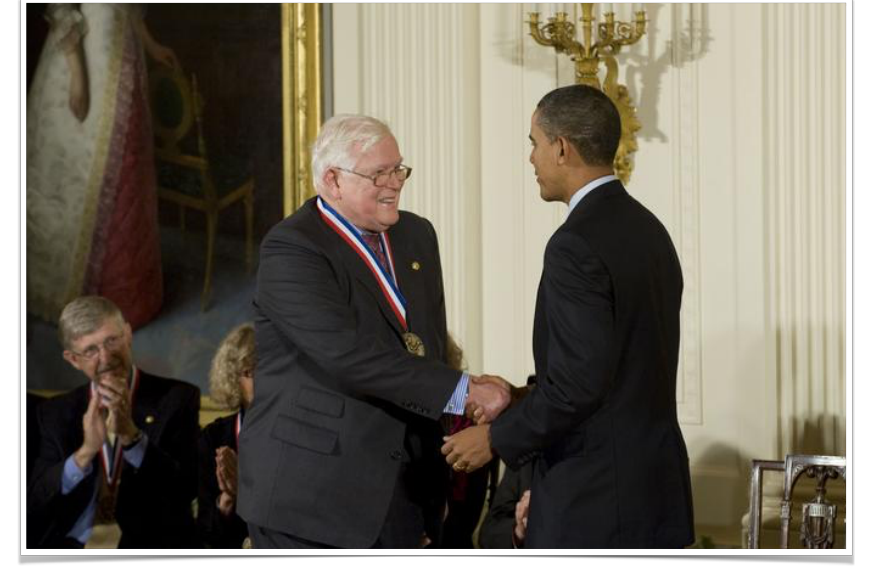
\includegraphics[scale=0.280]{img/kalman_filter/rudolf_e_kalman.jpeg}
\end{center}
\caption{Rudolf E. Kálmán receiving the National Medal of Science.}
\label{rudolf_e_kalman}
\end{figure}


In this section, we'll learn about one of the most famous algorithms in all of engineering; namely the Kalman filter. In today's world of
advanced machine learning, the Kalman filter remains
an important tool to fuse measurements from several sensors to estimate in real-time the state of a robotic system such
as a self-driving car. Concretely, in this section, we will introduce its basic linear formulation and also show  why the Kalman filter is the best linear unbiased
estimator. 

\section{Introduction}
\label{kalman_filter_introduction}

The Kalman filter algorithm was
published in 1960 by Rudolf E. Kalman, a Hungarian born professor
and engineer who was working at the Research Institute
for Advanced Studies in Baltimore Maryland. Years later in 2009, American President Barack
Obama awarded Kalman the prestigious National Medal
of Science for his work on the Kalman filter and other contributions to the field
of control engineering.

After its publication in 1960, the Kalman filter was adopted by NASA for use in
the Apollo guidance computer. 

\begin{figure}[!htb]
\begin{center}
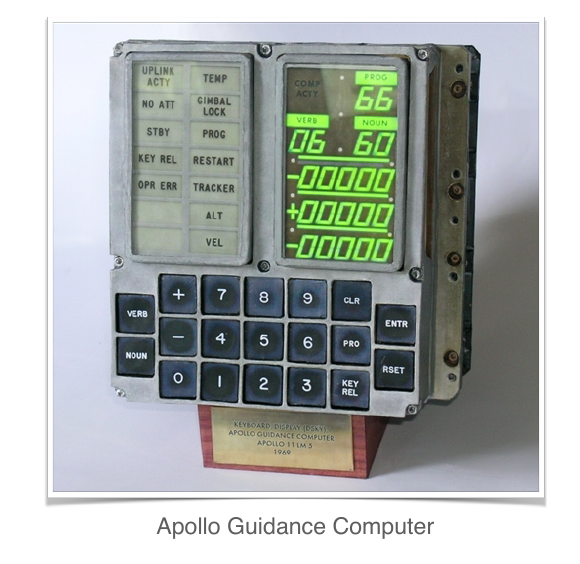
\includegraphics[scale=0.280]{img/kalman_filter/apollo_guidance_computer.jpeg}
\end{center}
\caption{The Apollo guidance computer used Kalman filtering.}
\label{apollo_guidance_computer}
\end{figure}

It was this ground-breaking innovation
that played a pivotal role in successfully getting
the Apollo spacecraft to the moon, and to our first steps on another world. The filter helped guide the Apollo spacecraft accurately
through its circumlunar orbit. 

The engineers at
NASA's Ames Research Center, adopted Kalman's linear theory and
extended it to nonlinear models. We will discuss this specific extension
in a later section. But first, let's talk about
the basic linear Kalman filter. 

\section{Linear Kalman Filter}


The Kalman filter is very similar to the linear recursive least squares
filter we discussed earlier. While recursive least squares updates
the estimate of a static parameter, but Kalman filter is able to update
and estimate of an evolving state. Thus, Kalman filtering is an iterative process that uses a set of equations and consecutive data inputs to quickly estimate the 
true value; e.g. position, velocity etc., of the object being measured when the measured values contain unpredicted or 
random error, uncertainty or variation.


The goal of the Kalman filter is to take a probabilistic estimate
of this state and update it in real time using
two steps; prediction and correction. 


To make these ideas more concrete, let's consider a problem of estimating
the 1D position of the vehicle. 

\begin{figure}[!htb]
\begin{center}
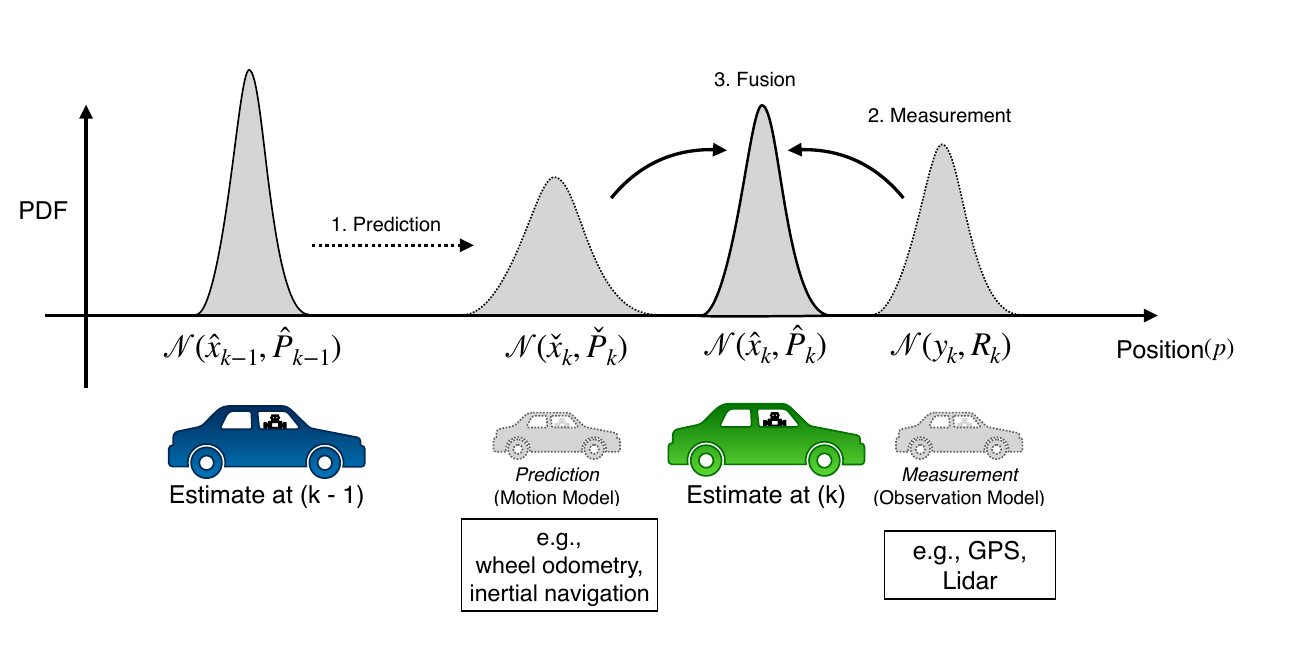
\includegraphics[scale=0.280]{img/kalman_filter/kalman_1.jpeg}
\end{center}
\caption{The Apollo guidance computer used Kalman filtering.}
\label{kalman_1}
\end{figure}

Starting from an initial probabilistic
estimate at time $k-1$, our goal is to use a \textbf{motion model}
which could be derived from wheel odometry or inertial sensor
measurements to predict our new state. Then, we'll use the observation model
derived from GPS for example, to correct that prediction
of vehicle position at time $k$. 

Each of these components, the initial estimate, the predicted state, and
the final corrected state are all random variables that we will specify
by their means and covariances. In this way, we can think of the Kalman filter as a technique to fuse information from
different sensors to produce a final estimate of some unknown state, taking into account, uncertainty
in motion and in our measurements. For the Kalman filter algorithm, we had been able to write
the motion model in the following way; the estimate at time step k is a linear combination of the estimate
at time step $k-1$, a control input and some zero-mean noise. 


The input is an external signal that affects the evolution of our system state. In the context of self-driving vehicles, this may be a wheel torque applied to speed up and change lanes, for example. Next, we will also need to define
a linear measurement model. Finally, we'll need a measurement
noise as before and a process noise that
governs how certain we are that our linear dynamical system
is actually correct, or equivalently, how uncertain we are about the effects
of our control inputs. 

\begin{eqnarray}
\mathbf{x}_k = \mathbf{F}_{k-1}\mathbf{x}_{k-1} + \mathbf{G}_{k-1}\mathbf{u}_{k-1} + \mathbf{w}_{k-1} \\
\mathbf{y}_k = \mathbf{H}_k \mathbf{x}_k + \mathbf{v}_k
\end{eqnarray}

where

\begin{equation}
\mathbf{v}_k \sim N(0, \mathbf{R}_k), ~~ \mathbf{w}_k \sim N(0, \mathbf{Q}_k) 
\end{equation}

Once we have our system in hand, we can use an approach
very similar to that we discussed in the recursive
least squares. Except this time, we'll
do it in two steps. 

\begin{itemize}
\item First, we use the process model to predict how our states, remember, that we're now typically talking
about evolving states and non-state parameters evolved since the last time step, and will propagate our uncertainty. 
\item Second, we'll use our measurement to correct that prediction based on our measurement residual
or innovation and our optimal gain. 
\end{itemize}

Finally, we'll use the gain to also propagate the state covariance from our prediction
to our corrected estimate. This is shown in Figure

\begin{figure}[!htb]
\begin{center}
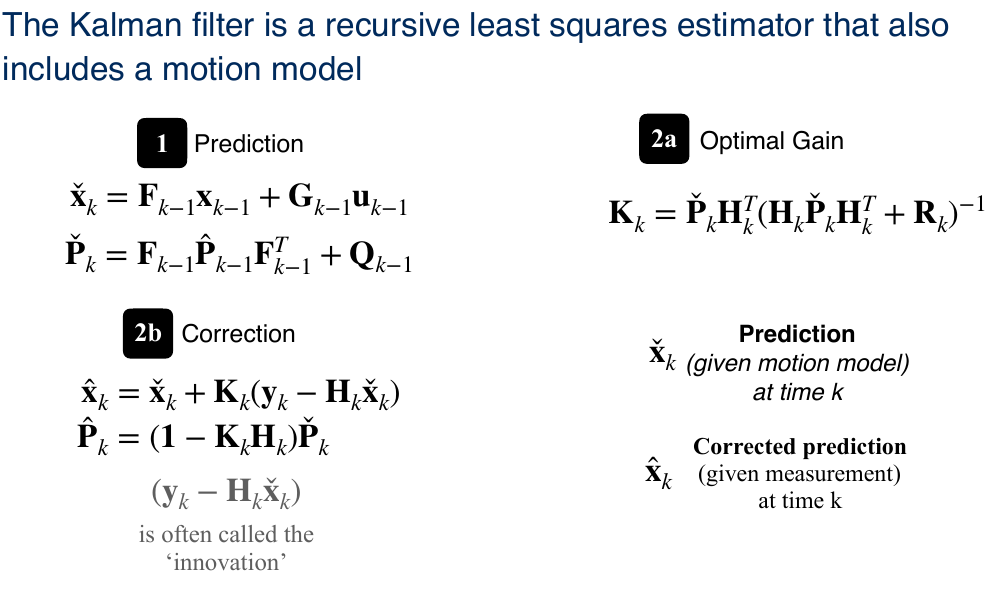
\includegraphics[scale=0.280]{img/kalman_filter/kalman_2.jpeg}
\end{center}
\caption{The linear Kalman filter steps.}
\label{kalman_2}
\end{figure}

In our notation, the hat indicates a corrected prediction
at a particular time step. Whereas a check indicates a prediction before
the measurement is incorporated. If you've worked with the
Kalman filter before, you may also have seen this
written with plus and minus signs for the corrected and
predicted quantities, respectively. 

Let's recap. We start with
a probability density over our states and also maybe parameters
at time step $k-1$, which we represent as
a multivariate Gaussian. We then predict the states
at time step $k$ using our linear prediction model and propagate both the mean
and the uncertainty; the covariance, forward in time. Finally, using our probabilistic
measurement model, we correct our initial
prediction by optimally fusing the information from
our measurement together with the prior prediction through our optimal
gain matrix $\mathbf{K}$. Our end result is an updated probabilistic estimate
for our states at time step $k$. 

\begin{figure}[!htb]
\begin{center}
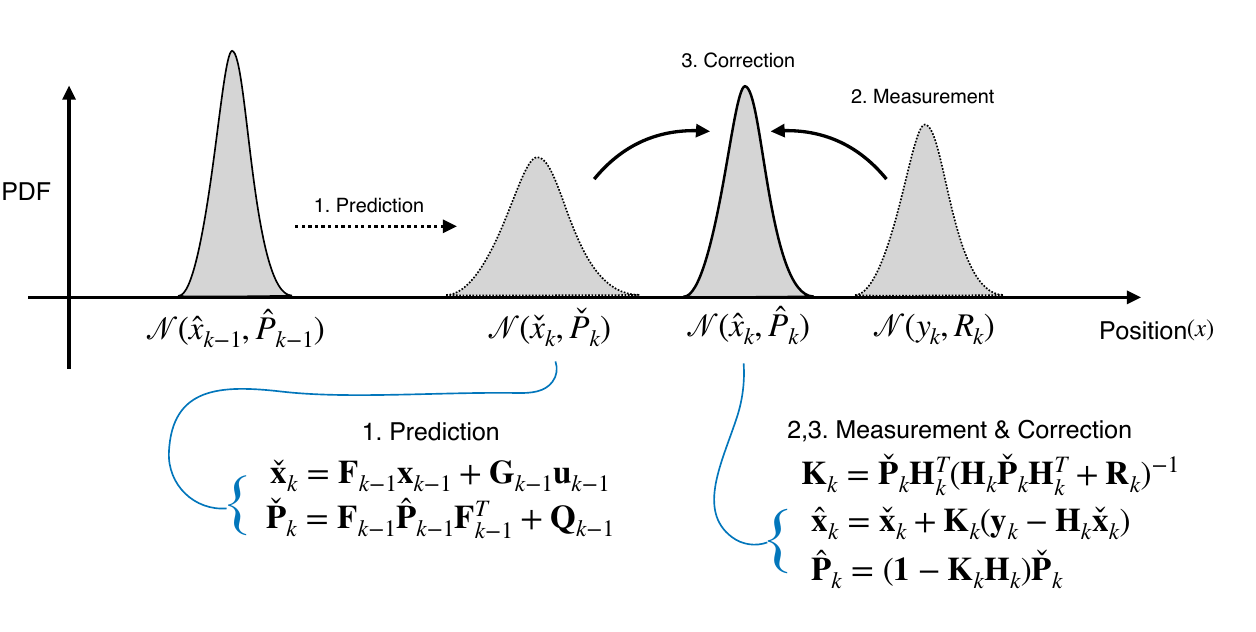
\includegraphics[scale=0.280]{img/kalman_filter/kalman_3.jpeg}
\end{center}
\caption{The linear Kalman filter steps.}
\label{kalman_3}
\end{figure}

\subsection{Example: 1D Vehicle Motion}

The best way to become comfortable with the
Kalman filter is to use it. Let's look at a simple example. Consider again the case of the self-driving vehicle
estimating its own position. Our state vector will include the vehicle position and
its first derivative velocity. Our input will be a scalar acceleration
that could come from a control system that commands our car
to accelerate forward or backwards. For our measurement, we'll assume
that we're able to determine the vehicle position directly using
something like a GPS receiver. Finally, we'll define
our noise variances as follows: Given this initial
estimate and our data, what is our corrected position
estimate after we perform one prediction step and one correction
step using the Kalman filter? Here's, how we can use
these definitions to solve for our corrected position
and velocity estimates. Pay attention to the fact that our final corrected state
covariance is smaller. That is we are more certain about the car's position after we
incorporate the position measurement. This uncertainty reduction occurs because our measurement model
is fairly accurate. That is, the measurement noise
variance is quite small. Try increasing
the measurement variance and observe what happens to
the final state estimate. To summarize, the Kalman filter is
similar to recursively squares, but also adds a motion model that
defines how our state evolves over time. The Kalman filter works
in two stages: First, predicting the next state
using the motion model, and second, correcting
this prediction using a measurement. But how can we be sure
that the Kalman filter is giving us an accurate state estimate? 


\section{Kalman Filter and BLUE}
\label{kalman_filter_blue}

We have introduced the Kalman Filter, let's discuss little bit about what makes
it such an appealing estimation method. 

\subsection{Bias}
\label{kalman_filter_bias}

Let's dive in. First, let's discuss bias. Let's consider our Kalman Filter
from the previous lesson and use it to estimate the position
of our autonomous car. If we have some way of knowing the true
position of the vehicle, for example, an oracle tells us, we can then use this to record a position
error of our filter at each time step $k$. Since we're dealing with random noise,
doing this once is not enough. We will need to repeat this same
process over and over and record our position
error at each time step. Once we've collected these errors, if they
average to zero at a particular time step $k$, then we say the Kalman Filter
estimate is unbiased at this time step.  Graphically, this is what the situation may look like. 

\begin{figure}[!htb]
\begin{center}
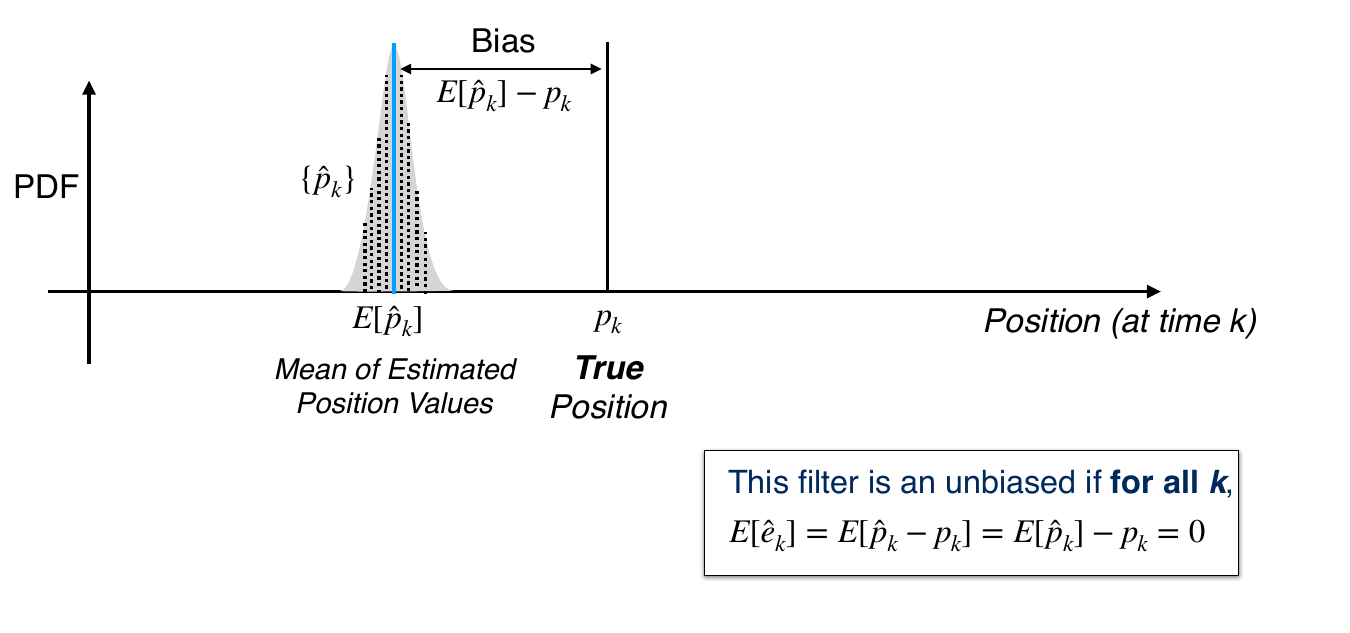
\includegraphics[scale=0.280]{img/kalman_filter/kalman_4.jpeg}
\end{center}
\caption{The linear Kalman filter steps.}
\label{kalman_4}
\end{figure}

Say the particular time step, we know that the true position is the following. We build a histogram of the positions that
our filter reports over multiple trials, and then compute the difference between
the average of these estimates and the true position. If this difference does not approach zero,
then our estimate is biased. However, if this difference does approach
zero as we repeat this experiment many more times, and
if this happens for all time intervals, then we say that our filter is unbiased. Although we could potentially verify
this lack of bias empirically, what we'd really like are some
theoretical guarantees. 

Let's consider the error dynamics of our filter. We define our predicted and corrected state
errors as follows

\begin{eqnarray}
\text{Predicted state error: }~~\check{\mathbf{e}}_k = \check{\mathbf{x}}_k - \mathbf{x}_k\\
\text{Corrected estimate error: }~~\hat{\mathbf{e}}_k = \hat{\mathbf{x}}_k - \mathbf{x}_k
\end{eqnarray}

We can then use the common filter equations to write
the following relations. 

\begin{eqnarray}
\check{\mathbf{e}}_k = \mathbf{F}_{k-1}\check{\mathbf{e}}_{k-1} - \mathbf{w}_k \\
\hat{\mathbf{e}}_k = (\mathbf{I} - \mathbf{K}_k\mathbf{H}_k)\check{\mathbf{e}}_k + \mathbf{K}_k\mathbf{v}_k
\end{eqnarray}

For the Kalman Filter, we can show the expectation value of
these errors is equal to zero exactly. Meaning that we can show

\begin{equation}
E[\check{\mathbf{e}}_k] = \mathbf{0}, ~~ E[\hat{\mathbf{e}}_k] = \mathbf{0}
\end{equation}

For this to be true, we need to ensure that our initial state estimate is unbiased and that our noise is white,
uncorrelated, with zero mean. While this is a great result for linear systems, remember that this doesn't guarantee that
our estimates will be error free for a given trial, only that the expected
value of the error is zero. 

\subsection{Consistency}
\label{kalman_filter_consistency}

Kalman Filters are also what is called consistent. By consistency we mean that for
all time steps $k$, the filter covariants $P_k$ matches the expected
value of the square of our error. 

\begin{figure}[!htb]
\begin{center}
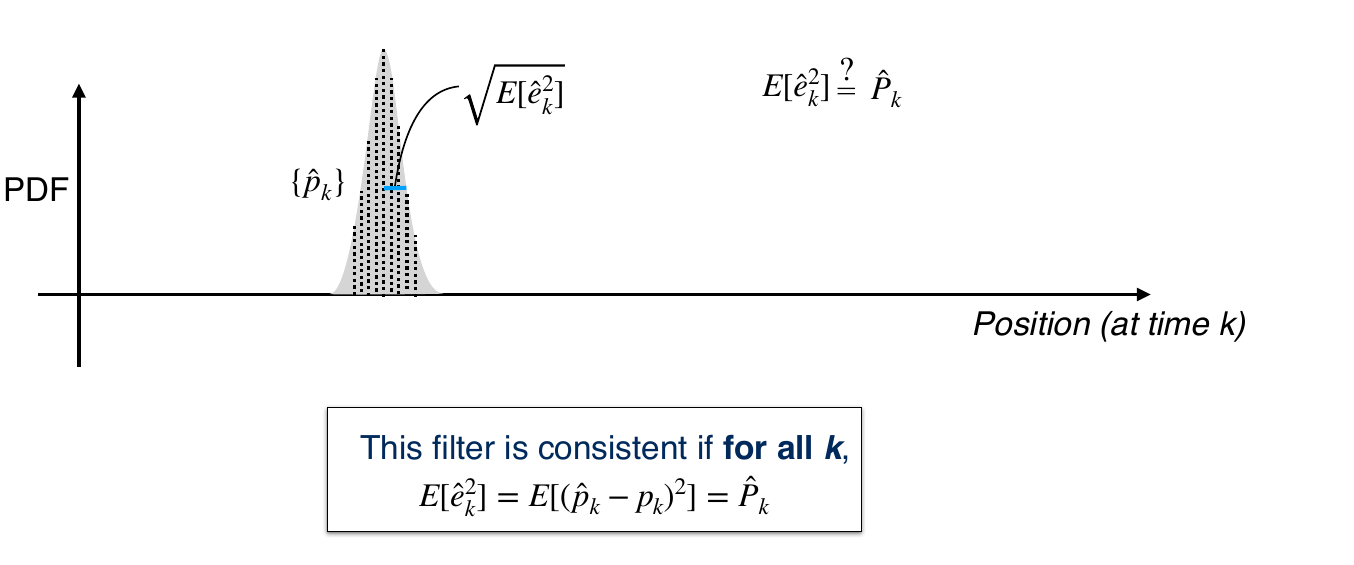
\includegraphics[scale=0.280]{img/kalman_filter/kalman_5.jpeg}
\end{center}
\caption{The linear Kalman filter steps.}
\label{kalman_5}
\end{figure}

For scalar parameters,
this means that the empirical variance of our estimate should match
the variance reported by the filter. Practically, this means that our
filter is neither overconfident, nor underconfident in
the estimate it has produced. 

\subsubsection{Overconfident filter}

A filter that is overconfident,
and hence inconsistent, will report a covariance
that is optimistic. That is, the filter will essentially place
too much emphasis on its own estimate and will be less sensitive to
future measurement updates, which may provide critical information. It's easy to see how an overconfident
filter might have a negative or dangerous effect on the performance
of self-driving car. 

So long as our initial
estimate is consistent, and we have white zero mean noise,
then all estimates will be consistent. Putting everything together,
we've shown that given white uncorrelated zero mean noise, the Kalman
Filter is unbiased and consistent. Because of these two facts, we say that the Kalman Filter is the BLUE,
the Best Linear Unbiased Estimator. It produces unbiased estimates with
the minimum possible variance. 

To summarize, in this section we've defined the terms bias and consistency, and
showed that the Kalman Filter is unbiased, consistent, and the Best Linear
Unbiased Estimator, or BLUE. Remember that best here refers to
the fact that the Kalman Filter minimizes the state variance. Although this is a fantastic result,
most real systems are not linear. For self-driving cars, we'll
generally need to estimate non-linear quantities like vehicle poses,
position, and orientation in 2D and 3D. To do this, we'll need to extend the linear
Kalman Filter into the non-linear domain. 


\subsection{Bayesian derivation of the Kalman filter}


So in the previous lecture, we presented a solution
to the filtering equations for linear and Gaussian models.
For these models, both the predicted
and the posterior density is Gaussian.
And the mean and covariance of these
are given by the Kalman filter equations.
Although we gave some hints in the previous lecture
for why the Kalman filter equations actually make sense,
in this lecture, we will more formally derive them,
and we will do so from a Bayesian perspective.
Before we start,
However, we need to define some prerequisites
and some notation.
So foremost, we assume that we have a linear and Gaussian
model.
So the state at the current type is
equal to the state at the previous time instance,
times this transition matrix, A k minus 1.
To account for added uncertainty in the predicted state,
we also have this additive noise process, q,
which is soon to be Gaussian with zero mean and covariance q
k minus 1.
The observation yk is similarly describe
as a linear function of the state, xk,
multiplied by this measurement model matrix, Hk.
And again, we have this additive noise process,
r, which we can assume to be Gaussian with zero mean
and covariance Rk In this case.
Additionally, we also need to assume that the prior state x
naught is also Gaussian, with some mean and some covariance.
We should also note that an equivalent
way of expressing these models here
is to express them on their density form
like this, where the process or motion model is defined
as a density over xk, where we know
the state at the previous time instance, xk minus 1.
And the measurement model or likelihood
is defined as a density over the observation yk
if we condition on the current state xk.
I would encourage you to make sure that you understand the
that these two express exactly the same thing, just
in two different ways.
So the objective of this lecture is
to use these models and the assumptions
that we presented here to derive analytical expressions
for the predicted density.
That is the density over xk given measurements up
to time k minus 1.
And for the posterior density, which
is then the density over xk, but now we also
condition on the measurement at the current time, k.
So there are many ways to derive the Kalman filter expressions.
One possible way is to derive the Kalman filter equations
from the filtering equations.
To do this, we simply plug in the Gaussian densities
that we presented in the previous slide
into these equations, and then try to solve them.
So for example, we need to calculate this integral here
and we need to solve this product here.
Although it's completely possible to do so,
unfortunately this involves various matrix manipulations,
and it's rather tedious.
So what we're going to present here
is a more standard derivation, where we instead
make use of well-known, or at least
well-known for statisticians, results regarding
Gaussian distributions.
Additionally, we hope that this will give you
some better understanding for what's happening in the Kalman
filter and help you understand a bit better
the non-linear filters that are based on the Kalman filter
that we will learn later on in this course.
Let's start with the prediction step.
So the objective here is to compute the predicted density.
And to do so, we use two assumptions.
First, we assume that the posterior density
from the previous time instance-- so the density
over xk minus 1, given measurements up to k minus 1,
is a Gaussian density with this mean and this covariance.
So remember that for our linear Gaussian models
all our filter densities are Gaussian.
And as a Kalman filter is a recursive filter,
this is a relevant assumption to make.
Secondly, we assume that we have a linear and Gaussian process
model like this that we presented
in the previous slide.
With this in mind, what we want to do
is use these assumptions to calculate the mean
and covariance of this density.
We will base our derivation on the well-known result
that if we have two independent Gaussian random variables--
let's call them z 1 and z 2 in this case.
A linear combination of these two variables
is then also Gaussian random variable, where
the mean is just a linear combination
of the mean of the these variables and the covariance
can be calculated like this, from the covariance
of the individual Gaussian random variables.
We can easily derive these expressions
by using fundamental rules for the expectation and covariance
operator that we have learned in the beginning of the course.
So as xk minus 1 and qk minus 1 are
independent Gaussian random variables,
we can use this result directly on our motion model
to get the predicted density.
So we want to calculate our predicted density, P of xk,
given measurements up to k minus 1,
which equals a Gaussian density of xk where the mean is given
by the expected value of xk, as described by this process
model, where we condition on observations up
to time k minus 1.
So we have ak minus 1 times the expected value
of xk minus 1, given measurements up to k minus 1,
which is exactly this mean here.

And then the expected value of qk minus 1 is just zero.
So it's zero mean.
So we get nothing else.
For the covariance, we again use this expression here.
So the covariance of xk minus 1, which is this covariance here,
is then multiplied by the transition
matrix on both sides.
We have Ak minus 1 times Pk minus 1, given k
minus 1 Ak minus 1 transpose, according to this formula here.
And then we need to add the covariance for our process
noise, qk minus 1.
So that's qk minus 1.

To map this to the notation that we have,
we call this mean, x hat k given k minus 1,
and we interpret this as the estimate of x at time k,
given observations up to k minus 1.
And similarly, for the covariance
we call this Pk given k minus 1, which
is the covariance of xk conditioned on measurements
up to k minus 1.
And we see that what we calculate here
is exactly what we calculate in the prediction
step of the Kalman filter.
So we have now derived the prediction step
in a Kalman filter.
Before we tackle the update step in the Kalman filter,
we need to understand an important lemma
for conditional distributions of Gaussian random variables.
And it goes like this.
So if x and y or two Gaussian random variables
with a joint probability density function like this--
so we concatenate x and y into single vector.
And that vector then is Gaussian distributed
with mean mu x and mu y, which is simply
the expected value of x.
And mu y is simply the expected value of y.
And that covariance matrix of this joint vector
here has this structure, where P of xx is the covariance of x.
And Pyy is then the covariance of y.
And Pxy is then the cross covariance of x and y.
We denote this as the covariance of x comma y.
And where Pyx is simply the cross covariance between y
and x, which is simply Pxy transpose,
as a covariance matrix needs to be symmetric.
So these need to be the transpose of each other.
And this cross covariance is then
related to how x and y are correlated
to each other or dependent on each other.
One should note that this structure here is general
and that we haven't made any other assumptions than that x
and y are jointly Gaussian.
So given that two variables are jointly Gaussian,
we can always structure its mean and covariance in this matter.
So based on this, the lemma states
that the conditional distribution of x given
y, for example, is then also Gaussian, where the mean is
given by the mean of x.
But we slightly shift it compared to the prior mean
of x, by this term here.
We further see that this term here
depends on the distance between the actual y
and what we expect y to be.
And that we wait this distance by a ratio
that it's dependent on how correlated x and y are,
divided by how much uncertainty we have in y.
As a sanity check, we can see that if Pxy is 0--
so x and y are uncorrelated.
We see that this term disappears and the mean
is simply the same as before.
So if we observed y and they are uncorrelated,
it doesn't change the mean of x, which is to be expected, right?
For the conditional covariance on the other hand,
again, we take the prior covariance of x, Pxx,
and then we reduce it by this factor here.
And here we can make two observations.
First, as with the conditional mean
if x and y are uncorrelated, so Pxy is zero.
This term again disappears and the covariance
of the conditional density is the same
as the covariance for x.
So observing y, and x and y are uncorrelated,
doesn't change the covariance of x.
It doesn't give us any information on x.
Second, if on the other hand x and y are correlated,
the covariance of x, if we conditional y,
will always be less than the covariance of x because we
reduce it by this factor here, and this factor here
is always positive.
And this also makes sense, right?
If they are correlated, after observing y,
we should be less uncertain about x than before we
made observation.
So in sum, the lemma states that if we have two jointly Gaussian
random variables, the conditional density is also
Gaussian with the mean and the covariance expressed like this.
Perhaps you can already now see some patterns here
for how we can use this lemma to prove the update
step in the Kalman filter.
But let's look at this in some more detail.
So when we do the update step in the Kalman filter,
we assume that we have already made the prediction
step that we showed earlier.
That is, we have computed the moments
of the predicted density of xk given observations up
to k minus 1.
And we denote these moments as this.
Additionally, we observe a measurement y
at time k, which is related to the state at time k
through this linear measurement model.
So here we have two Gaussian random variables.
And in order to see that they are jointly Gaussian,
it is convenient that we use the measurement model
and rewrite it to express the joint random variable x comma
y.
So we have this joint variable, xk yk,
which we want to express as something times xk
plus something times rk.
So we want to write it on this form here.
And in order for this to hold true,
we see that we need to have the identity matrix here
and we need to have a 0 here.
And this needs to be Hk.
And this needs to be the identity matrix.
So now we see that this equations holds true.
So xk is equal to xk plus 0 times rk.
And yk is equal to Hk xk plus rk, which is what we see here.
So now that we have written it on this form,
it actually follows directly that we
can write the joint distribution of xk yk
condition on all the measurements up to k minus 1
as this Gaussian density.
And it's perhaps useful to map this back
to the notation that was used in lemma on the previous slide.
So we have the expected value of x here.
So this was-- we call this mu x.
And this is then mu y.
This we called Pxx.

And this whole expression here, we call that Pyy.
And this was then the cross covariance between x and y.
And this here was then the cross covariance between y
and x, which is actually equal to the cross covariance
between x and y transposed.
Now if we use the lemma on conditional Gaussian densities,
we can express the posterior density
as this Gaussian density where the posterior mean, x hat k
given k, is equal to--
so if you use the lemma on the previous slide,
we see that we can form this as mu x plus Pxy times Pyy
inverse times y minus mu y.
So simply using the lemma on the previous slide,
we see that we can formulate the posterior mean
as this expression here.
And if we now identify what these
are from what we see here, we see
that this is equal to x hat k given minus 1
plus Pxy, this expression here, pk given k minus 1
and Hk transpose.
And then Pyy is this expression here.
Remember from the previous lecture,
we actually call this Sk as the innovation covariance.
So to simplify things, we will call it Sk in this equation.
So we have Sk inverse times y is yk in this case
minus the expected value of yk given observations
up to k minus 1, which is given here.
Hk times x hat k given k minus 1.
So if we look at this, we can see that this here--
this difference here is what we call the innovation
in the previous lecture.
And this factor here in front of it
is what we call the Kalman gain.
So this is actually equal to call Kalman gain
times the innovation.
And this is exactly how the updated mean is calculated
in the Kalman filter.
So how about the posterior covariance?
So again, if we use the lemma, we
see that our posterior covariance
can be written as Pxx minus cross-covariance x and y
times Pyy inverse times Pyx.

And Pyx, we see that this is just a transpose of Pxy.
So we exchange it like this.
So if we identify what things are here-- so Pxx
is just a predicted covariance.

And then, Pxy is this expression here.

And Pyy is just Sk, so Sk inverse.
And then Pxy transpose is just this expression here,
but transposed.

So now, if we introduce a small little trick saying that Sk
times Sk inverse--
so this product here is simply the identity matrix.
So we can insert this into our equation
here without changing anything.
So if we rewrite this as--

and then insert this identity matrix here
in the middle, which we can take the transpose of,
as it's a symmetric matrix.

We get the following expression.
And if we look at this, we can see that this factor here
is actually the Kalman gain.
And this factor here is simply the Kalman gain transposed.
So with this, we have that the updated covariance matrix
is simply the predicted covariance
minus the Kalman gain times the innovation
covariance times the Kalman gain transpose, which
is also exactly how we presented it in the previous lecture.
So now we have also derived the update step
of the Kalman filter.
We have now derived a Kalman filter
using some well-known results regarding Gaussian densities.
And you might wonder, why is this important?
Well, from my perspective, I think
it's important from at least two aspects.
First, being able to derive the Kalman filter
offers some intuition into what the Kalman filter actually
does.
And secondly, by being able to derive the Kalman filter,
we can figure out how we need to adapt equations
if the underlying assumptions changes slightly.
This could, for example, be if we no longer
have zero mean process and measurement noise,
how do we then need to adapt these equations in order to fit
this slightly different model?
We end this lecture with a self-assessment question
where you can try out your intuition regarding correlation
and the distribution of random variables.


\section{Kalman Filter Tuning}
\label{kalman_filter_tuning}

\section{Kalman Filter and LMMSE Estimators}



\subsection{Kalaman Gain}
The Kalman gain $K$is used to determine how much of the new measurements to use in order to update the new estimate.
In the caluclation of the Kalman gain two quantities participate:

\begin{itemize}
\item Error in estimate
\item Error in data measurement
\end{itemize}

Thus $K$ is given by

\begin{equation}
K = \frac{E_{est}}{E_{est} + E_{meas}}
\label{kalman_gain}
\end{equation} 

From equation \ref{kalman_gain} it follows that

\begin{equation}
0 \leq K \leq 1
\label{kalman_gain_condition}
\end{equation} 

The Kalman gain is the used used to update the current estimate $\hat{x}_t$:

\begin{equation}
\hat{x}_t = \hat{x}_{t-1} + K (z - \hat{x}_{t-1})
\label{new_estimate}
\end{equation} 


When $K \approx 1$ or is equal to one, the measurements we are getting a very accurate however the estimates are unstable. On the other hand when $K$ is small, 
the measurements we are getting a inaccurate but the estimates are stable since the error is small.
The error $E_{\hat{x}}$ in the estimate is given by 

\begin{equation}
E_{\hat{x}_t} = (1-K)E_{\hat{x}_{t-1}}
\label{estimate_error}
\end{equation}

\subsection{Calculations of Kalaman Filter}
The Kalman filter iterates over the following three calculations:

\begin{itemize}
\item Calculate $K$ using equation \ref{kalman_gain}
\item Calculate the new estimate using equation \ref{new_estimate} 
\item Caluclate the error in the estimate using equation \ref{estimate_error}
\end{itemize}

\subsubsection{Example: Temperature Estimate}


\section{Multidimensional Case}

Let's now turn attention to the multidimensional case. Let's introduce some notation. Let $X_0$ and $P_0$ be the initial state.
The matrix $X_0$ contains the initial state of the system. The matrix $P_0$ is the initial process covariance matrix. The process
covariance matrix represents the error in the estimate.


\begin{framed}
\theoremstyle{remark}
\begin{remark}{\textbf{Covariance Matrix}}

A covariance matrix, also known as auto-covariance matrix, dispersion matrix, variance matrix, or variance–covariance matrix, 
is a matrix whose element in the $i, j$ position is the covariance between the $i-th$ and $j-th$ elements of a random vector. 
A random vector is a random variable with multiple dimensions. 
Each element of the vector is a scalar random variable. 
Each element has either a finite number of observed empirical values or a finite or infinite number of potential values. 
The potential values are specified by a theoretical joint probability distribution. 
\end{remark}
\end{framed}



\begin{framed}
\theoremstyle{remark}
\begin{remark}{\textbf{Nonlinear Systems}}

The definition above holds for nonlinear systems as well, and the results discussed here have extensions to the nonlinear case.
\end{remark}
\end{framed}

One of the principal uses of observers in practice is to estimate the state of a
system in the presence of noisy measurements. We have not yet treated noise in our
analysis, and a full treatment of stochastic dynamical systems is beyond the scope
of this text. In this section, we present a brief introduction to the use of stochastic
systems analysis for constructing observers. We work primarily in discrete time to
avoid some of the complications associated with continuous-time random processes
and to keep the mathematical prerequisites to a minimum. This section assumes
basic knowledge of random variables and stochastic processes; see Kumar and
Varaiya [KV86] or Åström [Åst06] for the required material.

Consider again the LTI state-space model

\begin{equation}
\frac{dx}{dt} = Ax + Bu +v  ~~ y = Cx + Du +w 
\end{equation}
the model is augmented with additional terms representing the error or disturbance. Concretely,
$v$ is the process disturbance and $w$ is measurements noise. Both are assumed to be normally distibuted with zero mean;

\begin{eqnarray}
E[v] = 0, ~~ E[vv^T] = R_v, ~~ E[w] = 0, ~~ E[ww^T] = R_w 
\label{noise_proccess_1} 
\end{eqnarray}



\begin{framed}
\theoremstyle{remark}
\begin{remark}{\textbf{Normally distributed random variable}}

A one dimensional random variable $X$ is said to follow the normal distribution
\end{remark}
\end{framed}


\begin{framed}
\theoremstyle{remark}
\begin{remark}{\textbf{Nonlinear Systems}}

The definition above holds for nonlinear systems as well, and the results discussed here have extensions to the nonlinear case.
\end{remark}
\end{framed}

$R_v$ and $R_w$ are the covariance matrices for the process disturbance $v$ and the measurement noise $w$ respectively. Furthermore, we assume that the variables $v, w$ are not correlated i.e 

\begin{eqnarray}
E[vw^T] = 0
\label{noise_proccess_2} 
\end{eqnarray}


\begin{framed}
\theoremstyle{remark}
\begin{remark}{\textbf{Corralated random variables}}

Two random variables $X$ and $Y$ are said to be linearly correlated 
\end{remark}
\end{framed}

The initial condition is also modeled as a Gaussian random variable

\begin{eqnarray}
E[x(0)] = x_0, ~~ E[x(0)x^{T}(0)] = P_0
\label{noise_proccess_3} 
\end{eqnarray}

Implementation of the state-space model in a computer requires discretization. Thus the system can be written as discrete-time linear system with dynamics governed by

\begin{equation}
x_{t+1} = Ax_t + Bu_t + Fv_t,  ~~ y_t = Cx_t + w_t 
\end{equation}

Given the measurements $\{y(\tau), 0 \leq \tau \leq t \}$, we would like to find an estimate $\hat{x}_t$ that minimizes the mean square error:

\begin{equation}
E[(x_t - \hat{x}_t)(x_t - \hat{x}_t)^T] 
\end{equation}

\begin{framed}
\theoremstyle{theorem}
\begin{theorem}{\textbf{Kalman 1961}}


Consider the random process $x_t$ with dynamics described by  

\begin{equation}
x_{t+1} = Ax_t + Bu_t + Fv_t,  ~~ y_t = Cx_t + w_t \nonumber
\end{equation} 

and noise processes and initial conditions described by \ref{noise_proccess_1},  \ref{noise_proccess_2} and 
\ref{noise_proccess_3}. The observer gain $L$ that minimizes the mean square error is given by  

\begin{equation}
L_t = AP_tC^T(R_w + CP_tC^T)^{-1}  \nonumber
\end{equation}

where

\begin{equation}
P_{t+1} =  (A − LC)P_t(A − LC)^T + R_v LR_w L^T, ~~ P_0 = E[x_0x^{T}_0\}
\end{equation}

\end{theorem}
\end{framed}

A proof of this result can be found in \cite{Astrom}. We, note, however the following points:

\begin{itemize}
\item the Kalman filter has the form of a recursive filter: given mean square error $P_t$ at time $t$, we can compute how the estimate and error change. Thus we do not need to keep track of old values of the output.
\item Furthermore, the Kalman filter gives the estimate $\hat{x}_t$ and the error covariance $P_t$, so we can see how reliable the estimate is. 
It can also be shown that the Kalman filter extracts the maximum possible information about output data. 
If we form the residual between the measured output and the estimated output,
\end{itemize}

\begin{equation}
e_t = y_t - C\hat{x}_t
\end{equation}
we can show that for the Kalman filter the error covariance matrix $R_e$ is

\begin{equation}
R_e(i,j) = E(e_{j}e_{k}^{T}) = W_t\delta_{jk} 
\end{equation}

In other words, the error is a white noise process, so there is no remaining dynamic information content in the error.




\begin{framed}
\theoremstyle{theorem}
\begin{theorem}{\textbf{Kalman-Bucy 1961}}


The optimal estimator has the form of a linear observer 

\begin{equation}
\frac{d\hat{x}}{dt} = A\hat{x} + Bu + L(y - C\hat{x}),  ~~ \hat{x}(0) = E(x(0)) \nonumber
\end{equation} 

where $L$ is given by

\begin{equation}
L = PC^TR_{w}^{-1}  \nonumber
\end{equation}

where $P$

\begin{equation}
P(t) = E((x(t)-\hat{x}(t))(x(t)-\hat{x}(t))^T)  \nonumber
\end{equation}

\end{theorem}
\end{framed}


All matrices $A, B, C, R_v, R_w, P$ and $L$ can be time varying. The essential condition is that the Riccati equation (8.30) has a unique positive 
solution.

\section{Kalman’s Decomposition of a Linear System}

We have already seen that two fundamental properties
of a linear input/output system are:

\begin{itemize}
\item reachability 
\item observability
\end{itemize}

It turns out that these two properties can be used to classify the dynamics of a system. The key
result is Kalman’s decomposition theorem, which says that a linear system can be
divided into four subsystems:

\begin{itemize}
\item $\Sigma_{ro}$ which is reachable and observable
\item $\Sigma_{r\bar{o}}$ which is reachable but no observable 
\item $\Sigma_{\bar{r}o}$ which is not reachable but is observable
\item $\Sigma_{\bar{r}\bar{o}}$which is neither reachable nor observable
\end{itemize}


Thus, from the input/output point of view, it is only the reachable and observable
dynamics that matter.

\begin{framed}
\theoremstyle{remark}
\begin{remark}{\textbf{Kalman's decomposition for state-space}}

The general case of the Kalman decomposition is more complicated and requires some additional linear algebra; 
see the original paper by Kalman, Ho, and Narendra [KHN63]. The key result is that the state space can still be decomposed
into four parts, but there will be additional coupling so that the equations have the form 
\end{remark}
\end{framed}

\subsection{Questions}
\label{questions_kalman_filters}

\begin{enumerate}
\item Recall that $\hat{\mathbf{x}}_k = \hat{\mathbf{x}}_{k-1} + \mathbf{K}_k\mathbf{v}_k$ and that $\mathbf{v}_k = \mathbf{y}}_{k} + \mathbf{H}_k\hat{\mathbf{x}}_{k-1}$. Suppose that 
$y_k = x_k + r_k$ with $H_k = 1$ and $r_k \sim N(0,R)$. Which of the following statements apply?

\begin{enumerate}
\item if $R=\infty$ then $K_k \approx 0$
\item if $R=0$ then $K_k = \infty$
\item if $R=1$ then $K_k = 0$
\item if $R=0$ then $K_k = \infty$
\end{enumerate}
\end{enumerate}


\section{Answers}

\begin{enumerate}
\item Recall that $\hat{\mathbf{x}}_k = \hat{\mathbf{x}}_{k-1} + \mathbf{K}_k\mathbf{v}_k$ and that $\mathbf{v}_k = \mathbf{y}}_{k} + \mathbf{H}_k\hat{\mathbf{x}}_{k-1}$. Suppose that 
$y_k = x_k + r_k$ with $H_k = 1$ and $r_k \sim N(0,R)$. Which of the following statements apply?

\begin{enumerate}
\item if $R=\infty$ then $K_k \approx 0$
\item if $R=0$ then $K_k = \infty$
\item if $R=1$ then $K_k = 0$
\item if $R=0$ then $K_k = \infty$
\end{enumerate}

$R = \infty$  means the measurement is completely uninformative, and we should not trust it at all. Thus,
 the innovation should not be incorporated in the posterior, and we can note that achieves just that.
$R = 1 $ means the measurement is completely free from noise, and we can trust it completely. 
Thus, the innovation should be incorporated to 100% in the posterior, and we can note that achieves just that. 
If we get a , we have a problem, since that would mean we would take a step in the direction of 
the measurement that is longer than to the measurement itself. That would not make sense. Hence,  the first and the fourth options are the correct ones. 
\end{enumerate}


